\section{Three-phase buck-type rectifiers}
	
As  general case a front-end  converter power supply (e.g. lighting or telecommunications) shall designed that should have approximately these general characteristics: sinusoidal main currents, unity power factor, high power density and simplicity of the power circuit structure. Two structures are most fitted for the task. First a boost-type input rectifier (e.g., Vienna rectifier, \cite{kolar1996design}), that typically features two $400V$ output voltages with a three-level isolated  DC-DC  converter  or  two  isolated  DC-DC  output  stage (see Fig. \ref{EMPC:fig:network} in Ch.5.). The second candidate is the buck-type  input  rectifier (or current source rectifier (CSR))  (conventionally  six-switch topologies as proposed in \cite{zargari1993current}, \cite{sato1993state}) with only one two-level isolated  DC-DC  converter  output  stage.  Also the  input  stage  can be realized as a three-switch topology with considerably  lower  system  complexity  as  compared  to  the boost-type structure. In particular, the number of utilized active and passive components is much lower. Furthermore, there is no middle-point that has to be stabilized, as this is the case for the boost-type structures, making control and active filter design less complex. Further system advantages are the potential of direct start-up and the implicit over current protection in case of an output short circuit. Therefore, this topologies of high interest for many safety critical applications as such future electric aircraft, or automotive applications or as power supplies for process technology \cite{nussbaumer2007comprehensive}.
The three-switch buck rectifier topology was first proposed in \cite{malesani1987three}. In \cite{itoh1989steady} and \cite{tooth2000effects}, aspects of the system modulation and control have been treated. The application of the topology used as an active filter is discussed in \cite{salo2005three}.  The addition of a DC-DC output boost-stage has been proposed in \cite{baumannnew} in order to main- tain 400-V output voltage for a wide input voltage range and for the case of unbalanced mains as, e.g., the loss of one phase.

\subsection{Basic operation principles}

For the derivation of the relative on-times of the three buck transistors $S_i$ (with ) the following assumptions are made for clarity and facilitation of calculations:
\begin{itemize}
	\item The AC-side filter capacitor voltages ($u_{c_p}$, where $p\in\{1,2,3\}$) at the input of the CSR are sinusoidal and in phase with the main harmonic component of voltage.
	
	\begin{equation}
        \begin{array}{rcl}
            u_{c_1}&=&\widehat{u}_cos(\omega t)\\
						u_{c_2}&=&\widehat{u}_cos(\omega t-2\pi/3)\\
						u_{c_3}&=&\widehat{u}_cos(\omega t+2\pi/3),\\
        \end{array}
        \label{BASICMPC:equ:basic_LTI}
    \end{equation}
	where $\omega$ is the network voltage's angular velocity.
	
	\item The mains currents are assumed to be equal to the fundamental component of the rectifier input currents.
	\item The current in the DC output inductor $L_{dc}$ is not affected by the high frequency ripple due to the switching operation.
\end{itemize}

 For achieving ohmic mains behavior also in case of unbalanced fundamental harmonics conditions the explained modulation method can still be utilized, however, additionally the control structure presented in \cite{baumann2005novel} has to be employed. The
waveforms of the phase and line-to-line mains voltages are divided into twelve $30°$wide sectors shown in Fig.\ref{BASICCSR:fig:waves}. The following calculations are based on the analysis of the first sector which is characterized by the voltage harmonic phase relation. For the remaining sectors the calculations can be accomplished in an similar manner \ref{nussbaumer2007comprehensive}.

\begin{figure}[!ht]
        \centering
        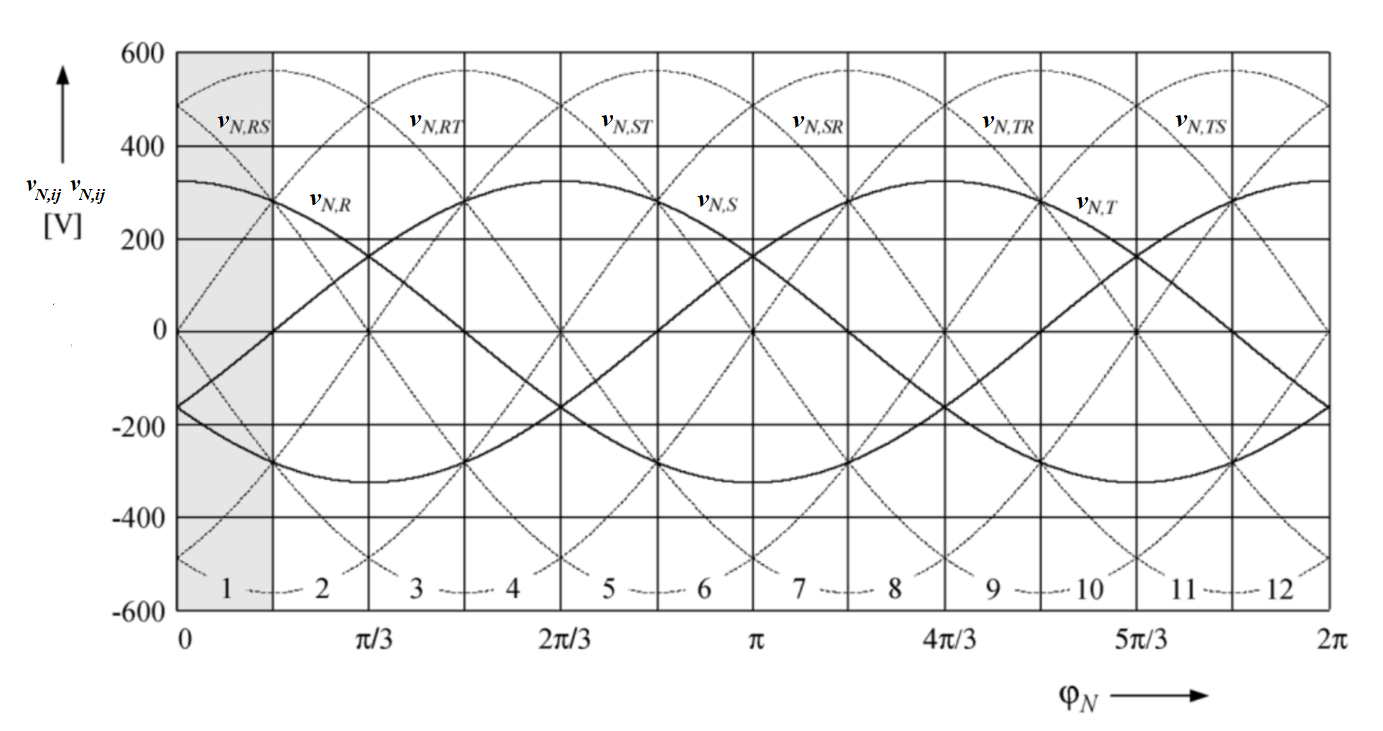
\includegraphics[width=\textwidth]{EMPC_PNG_Pics/Waves.png}
        \caption{Phase voltages $u_{i}$, where line-to-line voltages $u_{i,j}=u_i-u_j$, $(i,j)\in\{1,2,3\}$ and sectors $1–12$being defined by the different relations of the instantaneous values of the mains phase voltages for $u = 400 V$}
        \label{BASICCSR:fig:waves}
    \end{figure}
		
		Accordingly, on AC side, if conditions are favorable, inductor current can appear in an instant of time either in two out
of three phases or in none. In this modulation technique, the switches in each converter leg can conduct only one at the time (aside from zero states, where both upper and lower switches are conducting). When the upper leg is conducting it is indicated by `$1$', when the lower  `$-1$' and when neither `$0$'. As such the choice whether upper or lower switch of the leg conducts current depends of the reference current vector's sector location. 
According to the actual switch combination the DC link current shaped by the choke inductance, and distributed to two of the input phases or the freewheeling diode. With this, the input current space vectors can be calculated for each of the before-mentioned switching states. Generally the space vector of three-phase quantities (e.g., for the rectifier input current) are described as:

\begin{equation}
        \begin{array}{rcl}
            \vec{i}&=&\frac{2}{3}\left(\vec{i}_a+\vec{i}_be^{\frac{j\pi}{3}}+\vec{i}_bc^{\frac{4j\pi}{3}}\right).\\
        \end{array}
        \label{BASICCSR:eqn:currents}
    \end{equation}
		
		Based on \ref{BASICCSR:eqn:currents} the corresponding active space vectors in the first sector can be obtained as:
		
		\begin{equation}
        \begin{array}{rcl}
            \vec{i}_{(1,0,-1)}=\vec{i}_1&=&2i_{dc}e^{j\pi/6}/\sqrt{3}\\
						\vec{i}_{(0,1,-1)}=\vec{i}_2&=&2i_{dc}e^{j\pi/2}/\sqrt{3}\\
						\vec{i}_{(-1,1,0)}=\vec{i}_3&=&2i_{dc}e^{j5\pi/6}/\sqrt{3}\\
        \end{array}
        \label{BASICCSR:eqn:currents}
    \end{equation}
		
		The resulting discrete space vectors can be used to synthesize desired current
space vector $\vec{i}_{ref}$. 

The modulation methods were evaluated in and choosen for this paper based on \cite{moussaoui2005open}, which ensures minimum switching-losses, minimum ripple values of the input capacitor voltages and of the output inductor current. According to this modulation, each pulse interval comprises two active states and a freewheeling state, arranged symmetrically about the middle of the pulse interval (see Table \ref{EMPC:tbl:sequence}). For more in depth functional description see Chapter 5.

\section{Basis of quadratic optimization and model predictive control (MPC)}
	
	Predictive control methods based on a model are optimal regulators, with a defined cost function on a defined and encompassed  	prediction horizon with restrictions [N9], [N25], [N4], [N16], [N55]. The control signal is calculated over a defined horizon, but from the sequence of applicable control signals only the first one is used in the next sample. This procedure is repeated according to the principle of the moving horizon, using new iterations, as such provides the reaction in each sample. This method was developed for systems with physical restrictions, in the first stage for the control of chemical processes in the oil industry, then it was applied to various rapid processes from automotive or power electronics industry [N1] , [N13]. By default the optimization problem can be solved, for each sample, or explicitly using the multi-parameter programming techniques (mp-LP, mp-QP) presented in [N-ANNEX 1], over a well-defined parameter space.
	MPC example
	
	\subsection{Constained optimal control}
	
	Let the us assume that the system is linear and time-invariant (LTI):
	
	    \begin{equation}
        \begin{array}{rcl}
            x(t+1)&=&Ax(t)+Bu(t)\\
						y(t)&=&Cx(t)
        \end{array}
        \label{BASICMPC:equ:basic_LTI}
    \end{equation}
		
	with the restrictions:
	
	\begin{equation}
        \begin{array}{rcl}
            Ex(t)+Lu(t)\leq M\\
        \end{array}
        \label{BASICMPC:equ:restrict_LTI}
    \end{equation}
		
		where $t\geq0$ defines the time instance and $\textbf{x}\in \mathbb{R}^n$, $\textbf{u}\in \mathbb{R}^m$, $\textbf{y}\in \mathbb{R}^p$ are the states, inputs and outputs of the system respectively. We define the following cost function to optimize:
		
		\begin{equation}
        \begin{array}{rcl}
				%&&\norm{asd}
         J(U_n,x(0))&=&\norm{{Px_N}}_p+\sum^{N-1}_{k=0}\norm{Qx_k}_p+\norm{Ru_k}_p\\
        \end{array}
        \label{BASICMPC:equ:cost_function}
    \end{equation}
		
		The optimization problem \ref{BASICMPC:equ:cost_function} applies with restrictions as follows:
		
		\begin{equation}
        \begin{array}{rcl}
				J^*(x(0))&=&min_{U_N}J(U_n,x(0))\\
					&a.i.&Ex_k+Luk\leq M,k=0,\dots,N-1\\
					&&x\in X_f\\
					&&x_{k+1}=Ax_k+Bu_k,k\geq0\\
					&&x_0=x(0)\\
        \end{array}
        \label{BASICMPC:equ:optim_problem}
    \end{equation}
		%
		where $N$ is the defined horizon, $x\in X_f$ is the set if terminal states, $U_N=[u_0,u_1,\dots,u_{N-1}]\in\mathbb{R}^s,s=m*N$. In case of $p=2$ (Euclidean norm) $Q=Q'\geq0$, $R=R'\geq0$, $P\geq0$ and in case of $p=1$, $Q$,$R$, and $P$ shall be on maximum rank.
		From \ref{BASICMPC:equ:cost_function} and \ref{BASICMPC:equ:optim_problem} a classical linear quadratic regulator (LQR) structure can be formulated with finite or infinite horison [N3], [N20], [N21].
		Let us consider the following:
		
		\begin{equation}
        \begin{array}{c}
         p=2, \left\{(x,u)\in\mathbb{R}^n+m:Ex+Lu\leq M\right\}=\mathbb{R},X_f=\mathbb{R}^n\\
        \end{array}
        \label{BASICMPC:equ:quadratic_case}
    \end{equation}
		
		In this case the problem can be reduced to an unconstrained optimization with finite horizon with the control law: 
		
		\begin{equation}
        \begin{array}{rcl}
         u^*(k)&=&K_kx(k), k=0,\dots,N-1\\
        \end{array}
        \label{BASICMPC:equ:control_law}
    \end{equation}
		
		Where the control coefficient of the $k^th$ instance is $K_k$ can be given in the following form:
		
		\begin{equation}
        \begin{array}{rcl}
         K_k&=&-(B'P_{k+1}B+R)^-1B'P_{k+1}A\\
        \end{array}
        \label{BASICMPC:equ:control_coefficient}
    \end{equation}
		
		The positive semi-definite matrix $P_k$ is the solution of the Riccati equation:
		
		\begin{equation}
        \begin{array}{rcl}
        P_N&=&P\\
				P_k&=&A'(P_{k+1}-P{k+1}B(B'P_{k+1}B+R)^-1B'P_{k+1})A+Q\\
        \end{array}
        \label{BASICMPC:equ:Riccati}
    \end{equation}
		
		whith the initial condition:
		
		\begin{equation}
        \begin{array}{rcl}
				J^*(x(0))&=&x(0)'P_0x(0)\\
        \end{array}
        \label{BASICMPC:equ:Riccati_initial}
    \end{equation}
		
		If we choose $N\longrightarrow\infty$ and assume that $(A,B)$ are controllable and $(A,B)$ are observable, the optimization problem becomes an infinite horizon LQR whose solution can be written as:
		
		\begin{equation}
        \begin{array}{rcl}
         u^*(k)&=&K_kx(k), k=0,\dots,\infty\\
        \end{array}
        \label{BASICMPC:equ:control_law_infinite}
    \end{equation}
		
		As such:
		
		\begin{equation}
        \begin{array}{rcl}
         K_k&=&-(B'P_\infty B+R)^-1B'P_\infty A\\
        \end{array}
        \label{BASICMPC:equ:control_coefficient_infinite}
    \end{equation}
		
		with P as the unique solution of the Riccati equiation:
		
		\begin{equation}
        \begin{array}{rcl}
				P_\infty&=&A'(P_\infty-P\infty B(B'P_\infty B+R)^-1B'P_\infty)A+Q\\
        \end{array}
        \label{BASICMPC:equ:Riccati_infinite}
    \end{equation}
		
		These are the basis of model predictive control (MPC). For introduction let us consider the principle of moving horizon (Receding Horizon). Optimization over a finite horizon has the following disadvantages:
		
		\begin{itemize}
			\item Unforeseen problems may occur after the fixed optimization horizon, which may cancel the sequence of order for the 		calculated finished horizon.
		\item After reaching the time defined by the horizon, the law of command is no longer optimal.
		\item Finite horizon optimization is usually used because of the limited computing power is available, and not for theoretical reasons 
		\end{itemize}
		
		To prevent this problem, the notion of optimization is introduced on a moving horizon. In each sample $k$ , an optimization problem is solved over a defined horizon $k,\dots,k+N$ to calculate the appropriate command sequence, and only the first command is applied. This results in a moving optimization horizon, which eliminates the issues listed before. The Formulation of the optimal control problem with moving horizon [N14] in the system \ref{BASICMPC:equ:basic_LTI} with input and output constraints follows:
		
		\begin{equation}
        \begin{array}{c}
				y_{min}\leq y(t)\leq y_{max},u_{min}\leq u(t)\leq u_{max},\\
        \end{array}
        \label{BASICMPC:equ:receiding_horison_constraints}
    \end{equation}
		
		
with the cost function to minimize:
		
		\begin{equation}
        \begin{array}{rcl}
				J(U,x(t)&=&x'_{t+N_y|t}Px_{t+N_y|t}+\sum^{N_y-1}_{k=0}x'_{t+k|t}Qx_{t+k|t}+u'_{t+k}Ru_{t+k},\\
				&a.i.&y_{min}\leq y_{t+k|t}\leq y_{max},k=1,\dots,N_c-1,\\
				&&u_{min}\leq u_{t+k}\leq u_{max},k=0,1,\dots,N_c-1,\\
				&&x_{t|t}=x(t),\\
				&&x_{t+k+1|t}=Ax_{t+k|t}+Bu_{t+k},\\
				&&y_{t+k|t}=Cx_{t+k|t}, k\geq0,\\
				&&u_{t+k}=-Kx_{t+k|t}, N_u\leq k\leq N_y,\\
        \end{array}
        \label{BASICMPC:equ:receiding_horison_problem}
    \end{equation}
		
		where $Q=Q'\geq0$, $R=R'\geq0$, $P\geq0$, $(C,A)$ is observable, [missing text] and $N_u\leq N_y$, $N_c\leq N_y-1$. One trivial possibility to choose $K=0$ and $P$ to satisfy the Lyapunov equation:
		
		\begin{equation}
        \begin{array}{rcl}
				P&=&A'PA+Q\\
        \end{array}
        \label{BASICMPC:equ:receiding_horison_Lyapunov}
    \end{equation}
		
		This means that after $N_u$ samples the control stops and the system is evolving to an open loop form. It is obvious that the choice only makes sense if the open loop system is stable. The second option would as described in \ref{BASICMPC:equ:control_coefficient_infinite}, and \ref{BASICMPC:equ:Riccati_infinite}, but this involves to use an unconstrained control for $N_u$ LQR samples. As a result, the MPC law calculates the optimal command sequence:
		
		\begin{equation}
        \begin{array}{rcl}
				U^*(t)&=&\left\{u^*_t,\dots,u^*_{t+N_u-1}\right\},\\
        \end{array}
        \label{BASICMPC:equ:receiding_optimal_sequence}
    \end{equation}
		
		and only the first control input is applied:
		
		\begin{equation}
        \begin{array}{rcl}
				u(t)=u^*_t.\\
        \end{array}
        \label{BASICMPC:equ:receiding_optimal_first}
    \end{equation}
		
		The optimal control inputs estimated for future samples are not taken into account and the algorithm is
repeated on the basis of new measurements or a new estimation of the states.

\subsection{Stablilty of MPC}		
	
	The problem of closed system stability with the predictive control has been extensively studied e.g. in [N97], [N54]. In the first generation of model based controllers, stability was achieved more experimentally by choosing parameters based on previous studies and experiences. In 1988 Keerthi and Gilbert introduced the Lyapunov stability method for discrete systems [N65] , and in 1990 Mayne and Michalska for continuous systems [N96]. In this fashion, by using cost function, as a candidate for Lyapunov function, several methods of analysis have been developed, guaranteeing stability. 
	As basis the unconstrained LQR \ref{BASICMPC:equ:cost_function} is serving to create the Lypunov function such as:
	
\begin{equation}
        \begin{array}{rcl}
				V(x)&=&x'Px, P\succ 0.\\
        \end{array}
        \label{BASICMPC:equ:stability_Lyapunov_1}
    \end{equation}
		
	In order to test this lets make the following calculation:
	
	\begin{equation}
        \begin{array}{rcl}
				V(x_{k+1})-V(x_{k})&=&x'_{k+1}Px_{k+1}-x'_{k}Px_{k}=\\
				&=&k'_kA'PAx_k-x'_kPx_k=\\
				&=&x'_k(A'PA-P)x_k,\\
        \end{array}
        \label{BASICMPC:equ:stability_Lyapunov_2}
    \end{equation}
		
		where, in order to satisfy the Lyapunov theorem:
		
		\begin{equation}
        \begin{array}{rcl}
				A'PA-P&=&-Q, Q\succ 0.\\
        \end{array}
        \label{BASICMPC:equ:stability_Lyapunov_3}
    \end{equation}
		
	This is referred to as discrete-time Lyapunov equation, where  according to \cite{borrelli2017predictive} iff $P$ satisfying \ref{BASICMPC:equ:stability_Lyapunov_3}, then the system is asymptotically stable. From an optimisation point of view problem \ref{BASICMPC:equ:optim_problem} in compact form:
	
\begin{equation}
        \begin{array}{rcl}
				min_UJ(U,x)&=&F(x_N)+\sum^{N-1}_{k=0}L(x_k,u_k) \\
					&a.i.&x_{k+1}=f(x_k,u_k) \\
					&&x\in X, u\in U\\
					&&x_0=x(t)\\
        \end{array}
        \label{BASICMPC:equ:optim_stability}
    \end{equation}

Assuming that the function cost $J(U,x)$ is a Lyapunov candidate, the MPC would be asymptotically make the system stable, if the following conditions are met:
\begin{enumerate}
	\item There is a terminal set $\Omega\subset X$ so that $\Omega$ is also marginalized $0\in\Omega$ (contstraints of states are satisfied in $\Omega$).
	\item There is a terminal controller $K(x_k)\in U, \forall x\in\Omega,k=N,\dots,\infty$ (contstraints of inputs are satisfied in $\Omega$)
	\item The set $\Omega$ is invariant for the function $f(x_k,K(x_k)$ which needs to be optimized, so for every $x_0\in\Omega$, all subsequent $x_{k+1}=f(x_k,K(x_k)$ would remain in $\Omega$.
	\item $F(f(x_k,K(x_k)))-F(x)+L(x_k,K(x_k))\leq 0$, then $F()$ is the Lyapunov function in $\Omega$.
\end{enumerate}

Based on these conditions above, there are several methods of stabilizing the systems with MPC regulators, some of these are presented below [N16].

\begin{itemize}
	\item \textbf{MPC with final state constraint}: Stability is ensured by $x_N=0$. This imposes that $\Omega=\{0\}$, as such $K(x_k)=0$ maintains the state of origin. The advantage of the method is that we have a simple constraint, but imposing an equality constraint can to lead to difficulties in obtaining the solution.
	\item \textbf{MPC with terminal cost}: This method imposes a zero terminal cost, without imposing restrictions
for the final states. This method guarantees stability for large prediction horizons
of unrestricted systems.
	\item \textbf{MPC with permissible set restrictions of final states}: For this, it is required to $x_N\in\Omega$. This equality constraint ensures that the controller $K(x_k)$ remains in $\Omega$. This method is also called dual predictive controller, because two regulators are used, one with a moving horizon and one with stabilization of $K(x_k)$.
	\item \textbf{MPC with permissible set restrictions on final states and terminal cost}: Combined method, and widely used because it encompasses the advantages of previous methods.
\end{itemize}

There are also stabilization methods such as infinite horizon MPCs or suboptimal MPC regulators, but we do not detail these methods because they are not used in the thesis.

\section{Explicit model predictive control (EMPC)}

The problem \ref{BASICMPC:equ:receiding_horison_problem} can be transformed into a multi-parametric quadratic programming (mp-QP) problem. Such an approach involves solving the problem "offline", i.e. explicitly for the defined state-space with considering given constraints. By solving the optimization offline, critical regions are obtained, where each region corresponds to an optimal command that can be expressed as a function tuned by system states. Therefore the real-time regulation of the system is reduced to the identification of the critical regions corresponding to the measured state and the application of the optimal control input stored in a table. This method has revolutionized the use of the MPC method for systems with high dynamics, in particular for reduced order systems. The disadvantage of the method is that the number of critical regions increases exponentially with an increasing system order. The following shows the transformation of MPC into
mp-QP.
Let us assume an optimization problem described by \ref{BASICMPC:equ:receiding_horison_problem} The evolution of the subsequent states is calculated based on a mathematical of the system, according to the relation:

\begin{equation}
        \begin{array}{rcl}
				x_{t+k|t}&=&A^kx(t)+\sum^{k-1}_{j=0}A^jBu_{t+k-1-j}
        \end{array}
        \label{BASICMPC:equ:EMPC_evolution}
    \end{equation}

Based on \ref{BASICMPC:equ:receiding_horison_problem}, and \ref{BASICMPC:equ:EMPC_evolution} the optimization problem becomes:

\begin{equation}
        \begin{array}{rcl}
				V(x(t))&=&\frac{1}{2}x'(t)Yx(t)+min\left\{\frac{1}{2}U'HU+x'(t)FU\right\}\\
				&with\,restrictions:&GU\leq W+Ex(t)\\
        \end{array}
        \label{BASICMPC:equ:EMPC_transformed}
    \end{equation}
		
		where $U=\{u'_t,\dots,u'_{t+N_u-1}\}\in\mathbb{R}'s,\,s=m\cdot N_u$, $H$ is the optimization vector where $H=H'>0$, and $H,F,Y,G,W,E$ can be directly obtained from $A,B,Q,R,P$. Let the transfotmation variable be:
		
		\begin{equation}
        \begin{array}{rcl}
				z&=&U+H^{-1}F'x(t)
        \end{array}
        \label{BASICMPC:equ:EMPC_trans_var}
    \end{equation}
		
		the cost function \ref{BASICMPC:equ:EMPC_transformed} becomes:
		
		\begin{equation}
        \begin{array}{rcl}
				V(x)&=&V_z(x)+\frac{1}{2}x'\left(Y-FH^{-1}F'\right)x,
        \end{array}
        \label{BASICMPC:equ:EMPC_trans_var}
    \end{equation}
		
		where $V_z(x)$ is defined as:
		
		\begin{equation}
        \begin{array}{rcl}
				V_z(x)&=&min\frac{1}{2}z'Hz\\
				&s.t.&Gz\leq W+Sx(t)\\
				&with\,restrictions:&S=E+GH^{-1}F'.\\
        \end{array}
        \label{BASICMPC:equ:EMPC_transformed}
    \end{equation}
		
		From \ref{BASICMPC:equ:EMPC_transformed} the standartd mp-QP problem can be defined according to \cite{borrelli2017predictive}, and thorugh this transformation the MPC problem can be explicitly obtained. 
		

\subsection{Storage of critical regions}

The issue of iterative model based controllers is that they require a lot of computational resource. The CPU load and required ROM consumption could increase exponentially the longer the more steps the control horizon is calculated. For this reason explicit model bssed predictive controllers (EMPC) were developed, where only the storage the critical regions and the signal coefficients for each critical region, so the matrices $H$, $K$, $M$, $G$ are required. The on-line part of control consists of searching the critical region for the current states and calculating the necessary inputs for them.
One method of storing entire critical regions in order to calculate them, and that is in the order in which the MP-LP or MP-QP problem is resolved. It has the disadvantage, that the search time can be high, as such starting from the top of the list, a linear search is not effective. The efficient method is to store critical regions already in a binary tree [N64], [N111], [N23], [N113]. The method of generating the binary tree is shown in (Fig.\ref{BASICMPC:fig:searchtree}.). The basic idea is to sort the critical regions
depending on their adjacent sides. For example, in (Fig.\ref{BASICMPC:fig:searchtree}.a.) side $j_1$ divides the state space into two, at the right of it are the regions $X_{2,3,4,5}$ and to the left are the regions $X_{1,2,6}$. They make up the nodes adjacent to the base node $I_1$ of the binary tree. Next the another side from the space is choosen defined by each node $I_2$ respectively $I_3$, and the algorithm is continued until all the regions in the current node correspond to the same control signal, denoted by $F$ on the shaft in fig. (Fig.\ref{BASICMPC:fig:searchtree}.b.) Thus with this search pattern logarithmic search time can be achieved.

 \begin{figure}[!ht]
        \centering
        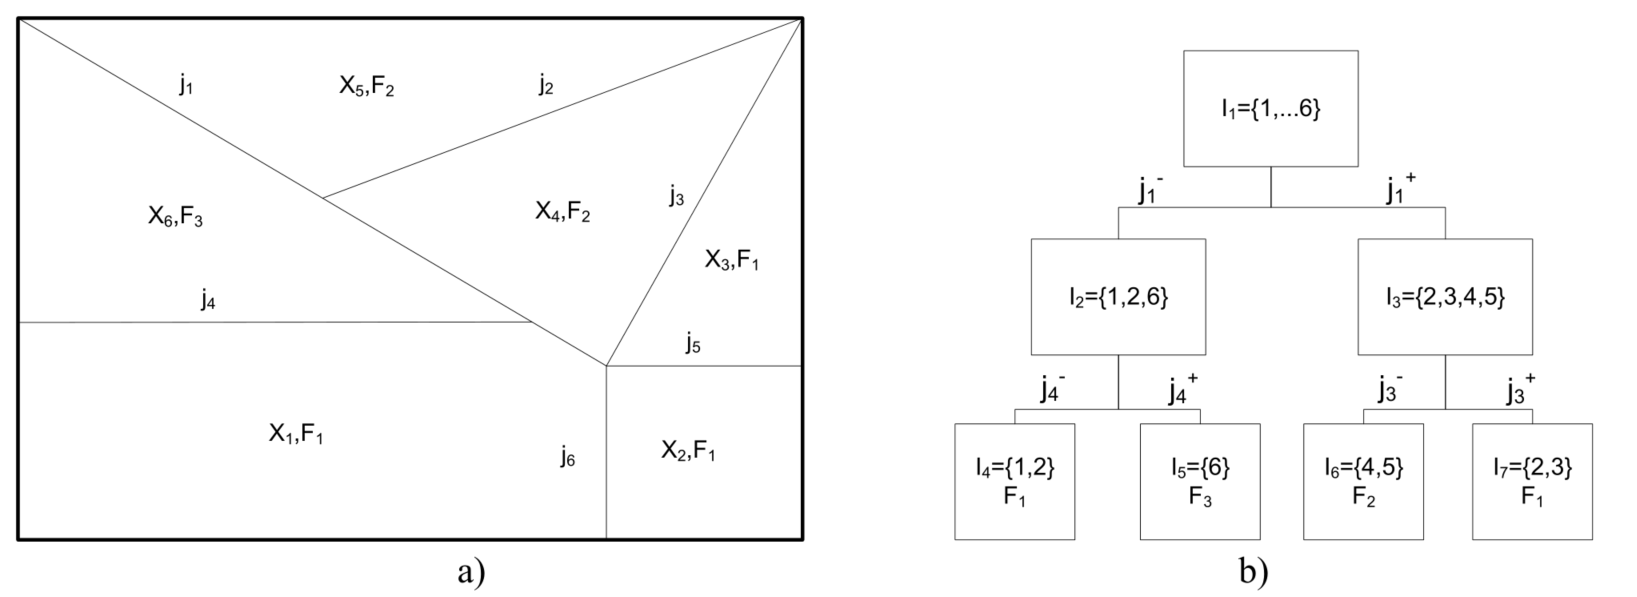
\includegraphics[width=\textwidth]{EMPC_PNG_Pics/BasicSearchTree.png}
        \caption{Basic search three of an EMPC where, a) are the critical regions for a space of 2D parameters,
b) the related binary tree.}
        \label{BASICMPC:fig:searchtree}
    \end{figure}

The implementation of MPC in explicit form is very efficient up to a certain number of critical regions, because they do not require calculations but only search in a table. For more complex problems or fast systems the method requires longer search time.

%\section{Summary}
%
%$\longmapsto$Summary of basic notions general.

